\chapter{The model hierarchy: order parameters, gradient flows, and scales}
\label{ch:p0}

\begin{keybox}
\textbf{Key idea.} Every model in this course is a \emph{gradient flow of a
free-energy functional}: the film evolves so as to decrease a single free
energy $F$, and the \emph{only} question that distinguishes one model from
the next is which fields are conserved, what free energy they minimize, and
how fast. Two dynamics cover everything --- \emph{conserved}
(Cahn--Hilliard, for composition) and \emph{non-conserved} (Allen--Cahn,
for crystallinity) --- and the eight concepts of the Physics track are the
same two dynamics with ingredients added one at a time. This chapter fixes
the vocabulary, the symbols, and the \emph{scales}: it derives the two
dynamics from $F$, works one nondimensionalization through in full, and
separates the four kinds of parameter (dimensional material data,
nondimensional groups, numerical knobs, and deliberately \emph{accelerated}
tutorial settings) that the rest of the course keeps apart.
\end{keybox}

\section{Conserved vs non-conserved order parameters}

An \emph{order parameter} is a coarse-grained field that labels the local
state of the film. This course uses two kinds, and the distinction governs
the dynamics:
\begin{itemize}[nosep]
  \item A \textbf{conserved} order parameter is a \emph{composition}: a
        local volume fraction $\phi$ (or $\phi_1,\phi_2,\dots$ for several
        species). Matter is neither created nor destroyed, so the spatial
        integral $\intv\phi\dV$ is fixed --- composition can only be
        \emph{redistributed}. Its dynamics must be a divergence of a flux
        (a local conservation law).
  \item A \textbf{non-conserved} order parameter is a \emph{degree of
        internal order}: the local crystallinity $\psi\in[0,1]$. Crystal
        can be \emph{created} (an amorphous region orders) or destroyed (it
        melts), so $\intv\psi\dV$ is \emph{not} fixed. Its dynamics is a
        direct relaxation, with no conservation constraint.
\end{itemize}

\begin{keybox}
\textbf{The test.} Ask ``can the spatial average change on its own?'' For
composition, no (it takes a flux through the boundary) --- \emph{conserved},
Cahn--Hilliard. For crystallinity, yes (it grows in place) ---
\emph{non-conserved}, Allen--Cahn. The moving-frame evaporation concepts
(\ref{ch:p5}, \ref{ch:p9}) are the one subtlety: the \emph{solvent} leaves
through the top surface, so a species' amount is conserved only in the
\emph{moving} film frame, and the bookkeeping is a per-species moving-domain
balance, not a fixed integral.
\end{keybox}

\section{Both dynamics are gradient flows of one free energy}

The organizing principle is a single Ginzburg--Landau free energy. For a
composition field it is
%
\begin{equation}
  F[\phi] = \intv\Big[\, f(\phi) + \tfrac{\kappa}{2}\,|\grad\phi|^2 \,\Big]\dV ,
  \label{eq:p0F}
\end{equation}
%
a \emph{bulk} (mixing) energy density $f$ that is minimized by the pure
phases, plus a \emph{gradient} penalty $\tfrac{\kappa}{2}|\grad\phi|^2$ that
charges for spatial variation and so sets a finite interface width. The
\emph{chemical potential} is the variational derivative
$\mu=\delta F/\delta\phi = f'(\phi)-\kappa\grad^2\phi$.

\paragraph{Conserved dynamics (Model B, Cahn--Hilliard).}
Because $\phi$ is conserved, it can only move down a flux; the natural,
thermodynamically consistent choice is a flux proportional to
$-\grad\mu$, so that
%
\begin{equation}
  \dd{\phi}{t} = \grad\!\cdot\!\big(M\,\grad\mu\big),
  \qquad \mu = f'(\phi) - \kappa\,\grad^2\phi ,
  \label{eq:p0ch}
\end{equation}
%
with mobility $M>0$. This is the \textbf{Cahn--Hilliard} equation. It
guarantees two things at once: mass conservation (the right-hand side is a
divergence, so $\dd{}{t}\!\intv\phi\dV=0$ under no-flux boundaries) and
energy decrease.

\paragraph{Non-conserved dynamics (Model A, Allen--Cahn).}
Crystallinity has no conservation constraint, so it relaxes
\emph{directly} down the energy gradient,
%
\begin{equation}
  \dd{\psi}{t} = -L_\psi\,\frac{\delta F}{\delta\psi}
              = -L_\psi\Big[\dd{f_{\text{cr}}}{\psi} - \varepsilon^2\grad^2\psi\Big],
  \label{eq:p0ac}
\end{equation}
%
with kinetic coefficient $L_\psi>0$ and crystalline gradient penalty
$\varepsilon^2$. This is the \textbf{Allen--Cahn} equation.

\begin{keybox}
\textbf{Why both decrease $F$ --- the gradient-flow guarantee.} For either
dynamics, the chain rule gives $\dd{F}{t}=\intv\frac{\delta F}{\delta u}\,
\dd{u}{t}\dV$. Substituting the two flows:
\begin{itemize}[nosep]
  \item Cahn--Hilliard: $\dd{F}{t}=-\intv M\,|\grad\mu|^2\dV \le 0$;
  \item Allen--Cahn: $\dd{F}{t}=-\intv L_\psi\,\big(\tfrac{\delta F}{\delta\psi}\big)^2\dV \le 0$.
\end{itemize}
$F$ is a \emph{Lyapunov functional} --- it can only decrease --- for both.
The difference is purely the constraint: the conserved flow moves mass
\emph{between} regions to lower $F$; the non-conserved flow changes the
field \emph{in place}. This single fact --- ``the film descends one free
energy'' --- is the thread through every concept.
\end{keybox}

\paragraph{The kinetic reading.} $M$ and $L_\psi$ set only \emph{how fast}
the descent proceeds, not \emph{where} it ends: the equilibrium morphology
is a property of $F$ alone (the wells of $f$, the penalties $\kappa$,
$\varepsilon^2$), while $M$ and $L_\psi$ set the time scale. For
crystallization the driving force also carries a \emph{sign}: below the
melting point the crystal well is lower and $\psi$ grows; above it, the
amorphous well is lower and $\psi$ melts (Chapter~\ref{ch:p6}).

\section{Why Cahn--Hilliard is fourth order, and the mixed formulation}

Substituting $\mu=f'(\phi)-\kappa\grad^2\phi$ into \eqref{eq:p0ch} gives a
single equation
%
\begin{equation}
  \dd{\phi}{t} = \grad\!\cdot\!\Big(M\,\grad\big[f'(\phi)-\kappa\grad^2\phi\big]\Big),
\end{equation}
%
whose highest term is $-M\kappa\,\grad^4\phi$: Cahn--Hilliard is a
\textbf{fourth-order} PDE (Allen--Cahn, by contrast, is second order). A
standard $C^0$ finite-element basis --- continuous, but with discontinuous
gradients across element faces --- cannot represent a fourth-order operator
directly (the weak form would need integrable second derivatives, i.e.\ a
$C^1$ basis, which is expensive in 2-D/3-D).

\begin{keybox}
\textbf{The mixed formulation.} Rather than a $C^1$ basis, split the
fourth-order equation into \emph{two coupled second-order} equations by
keeping $\mu$ as an independent unknown:
%
\begin{equation}
  \dd{\phi}{t}=\grad\!\cdot\!(M\grad\mu), \qquad
  \mu = f'(\phi) - \kappa\grad^2\phi .
\end{equation}
%
Now each equation has at most a Laplacian, so a $C^0$ basis suffices ---
at the cost of carrying \emph{two} fields per node, $(\phi,\mu)$, in a
node-major $2$-dof block. This is the ``mixed $(\phi,\mu)$ form'' the solver
uses everywhere; Chapter~\ref{ch:c0} traces its element residual and the
four $2\times2$ Jacobian blocks to code, and Chapter~\ref{ch:c1} verifies it
converges at the right order in \emph{both} fields.
\end{keybox}

\section{The model hierarchy}

Figure~\ref{fig:p0hierarchy} is the map of the whole Physics track: eight
concepts, each adding \emph{one} physical ingredient to the same
gradient-flow skeleton. Read top to bottom, it is the arc from the simplest
demixing to a full evaporation-conditioned crystallizing blend.

\begin{figure}[h]\centering
  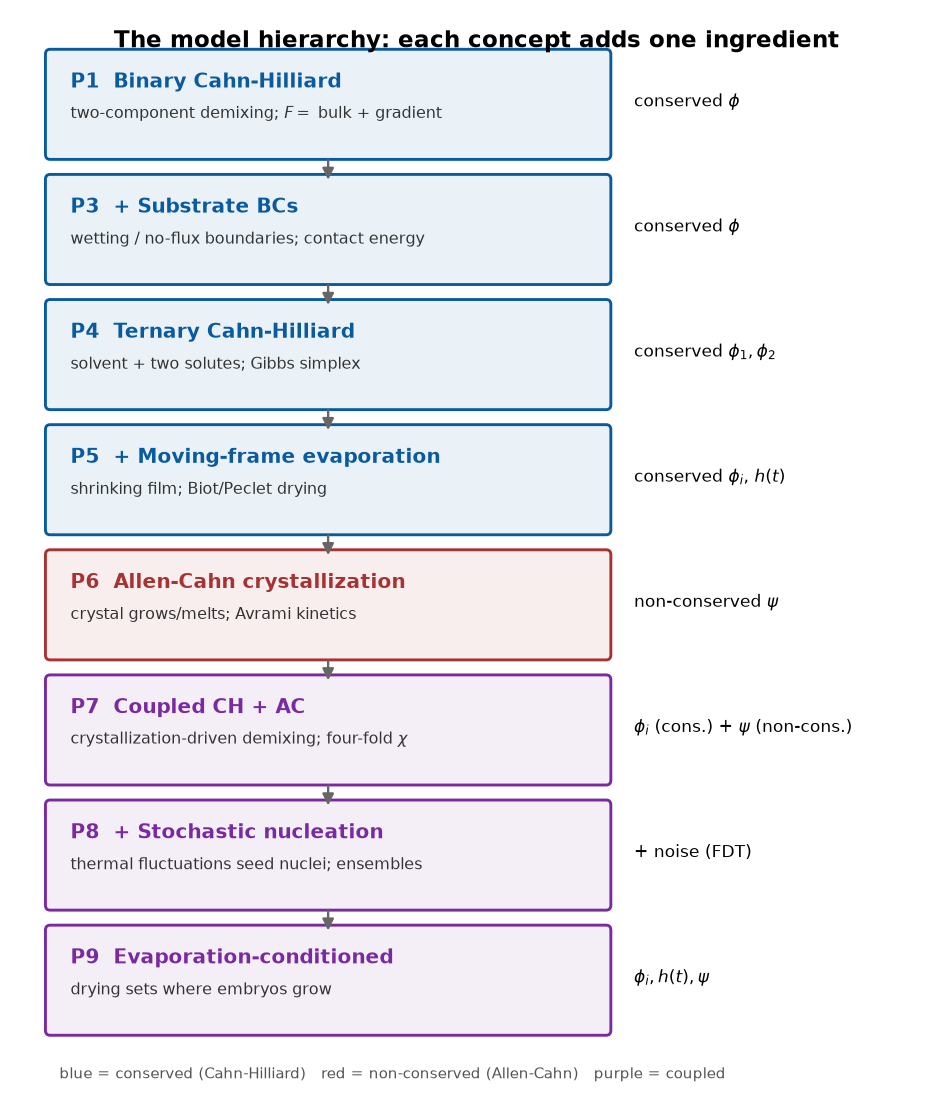
\includegraphics[width=\linewidth,height=0.88\textheight,keepaspectratio]{figures/p0_hierarchy.png}
  \caption{The model hierarchy. Blue = conserved (Cahn--Hilliard) fields;
    red = non-conserved (Allen--Cahn); purple = coupled. Each concept adds
    one ingredient: substrate boundaries, a third component, a moving
    (drying) frame, crystallinity, the coupling between composition and
    crystallinity, stochastic nucleation, and finally the
    evaporation-conditioned growth that ties them together.}
  \label{fig:p0hierarchy}
\end{figure}

\begin{itemize}[nosep]
  \item \textbf{Binary CH} (\ref{ch:p1}): two components demix; the base
        case. \;$\to$\; \textbf{$+$ substrate BCs} (\ref{ch:p3}): wetting
        and no-flux boundaries.
  \item \textbf{Ternary CH} (\ref{ch:p4}): solvent $+$ two solutes on the
        Gibbs simplex. \;$\to$\; \textbf{$+$ moving-frame evaporation}
        (\ref{ch:p5}): the film shrinks as solvent leaves.
  \item \textbf{Allen--Cahn crystallization} (\ref{ch:p6}): a non-conserved
        crystallinity field. \;$\to$\; \textbf{coupled CH$+$AC}
        (\ref{ch:p7}): crystallization drives demixing.
  \item \textbf{$+$ stochastic nucleation} (\ref{ch:p8}): thermal noise
        seeds nuclei. \;$\to$\; \textbf{evaporation-conditioned}
        (\ref{ch:p9}): drying decides where embryos grow.
\end{itemize}

\section{Symbol table}

\begin{center}\small
\begin{tabular}{lll}
\toprule
symbol & meaning & type / units \\
\midrule
$\phi,\ \phi_i$ & composition (volume fraction) & conserved, dimensionless \\
$\mu$           & chemical potential $\delta F/\delta\phi$ & energy/volume \\
$\psi$          & crystallinity & non-conserved, $\in[0,1]$ \\
$h(t)$          & film height (moving frame) & length \\
$F$             & Ginzburg--Landau free energy & energy \\
$f(\phi)$       & bulk (mixing) energy density & energy/volume \\
$f_{\text{cr}}(\psi)$ & crystallization energy density & energy/volume \\
$\kappa$        & composition gradient penalty & energy/length \\
$\varepsilon^2$ & crystalline gradient penalty & energy$\cdot$length \\
$M$             & Cahn--Hilliard mobility & sets composition time scale \\
$L_\psi$        & Allen--Cahn kinetic coefficient & sets crystal time scale \\
$W$             & bulk-energy barrier height (well depth) & energy/volume \\
$\ell$          & equilibrium interface width $\sim\!\sqrt{\kappa/W}$ & length \\
$\chi$          & Flory interaction parameter (enthalpic) & dimensionless \\
$N,\ N_i$       & degree of polymerization (entropic $\sim1/N$) & dimensionless \\
$A,\ B$         & FH entropy ($\sim1/N$) / enthalpy ($\sim\chi$) scales & dimensionless \\
$\Delta h$      & crystallization enthalpy (latent heat) & dimensionless \\
$\Delta\sigma$  & amorphous--crystal barrier & dimensionless \\
$T_m$           & melting temperature & K \\
$\mathrm{Bi}$   & Biot number $k_e h_0/D_s$ (evaporation rate) & dimensionless \\
$\mathrm{Pe}$   & P\'eclet number (advection/diffusion) & dimensionless \\
$\tilde\kappa$  & Cahn number $(\ell/L)^2=\kappa/(e_0L^2)$ & dimensionless \\
$\sigma$        & BDF time coefficient $b_0/\Delta t$ & 1/time \\
$L$             & domain size (length scale) & length \\
$e_0=kT/v_0$    & bulk free-energy scale ($v_0$ monomer volume) & energy/volume \\
\bottomrule
\end{tabular}
\end{center}

\section{Four kinds of parameter --- keep them apart}

A recurring source of confusion is mixing four \emph{different} kinds of
number. The course keeps them in separate tables, and so should you.

\paragraph{(1) Dimensional material parameters.} Physical properties of a
real blend, with units and a literature source. These live in
\file{materials/materials.yaml} with provenance.
\begin{center}\small
\begin{tabular}{llll}
\toprule
parameter & example (system) & value & source \\
\midrule
$\chi$ (polymer:fullerene) & P3HT:PCBM & $0.86$ & Wodo--Gan.\ CMS 2012 \\
$N$ (polymer) & PDPP5T:PCBM & $87$ & Negi et al.\ \\
$T_m$ (melting) & PCBM class & $\PzeroTm$~K & 2310.11844 Table~1 \\
$\Delta h$ (latent heat) & PCBM class & $1.31$ & 2310.11844 \\
$\mathrm{Bi}$ (evaporation) & PDPP5T @ 3000 rpm & $0.0051$ & Negi SI \\
\bottomrule
\end{tabular}
\end{center}

\paragraph{(2) Nondimensional groups.} The dimensionless combinations that
actually govern the solution --- the numbers a nondimensionalization
produces. Binary CH has \emph{one}: the Cahn number
$\tilde\kappa=(\ell/L)^2$. Evaporation adds the Biot and P\'eclet numbers;
crystallization adds the reduced undercooling $T/T_m-1$ and the barrier and
enthalpy ratios.
\begin{center}\small
\begin{tabular}{lll}
\toprule
group & meaning & tutorial value \\
\midrule
$\tilde\kappa$ (Cahn) & $(\ell/L)^2$; interface-to-domain ratio squared & $\PzeroCahn$ \\
$A,\,B$ (FH) & entropy $\sim1/N$, enthalpy $\sim\chi$ & $1.0,\ 2.5$ \\
$T/T_m-1$ & reduced undercooling (crystal drive sign) & $<0$ (grow) \\
$\mathrm{Bi},\ \mathrm{Pe}$ & evaporation rate, advection/diffusion & Ch.~\ref{ch:p5} \\
\bottomrule
\end{tabular}
\end{center}

\paragraph{(3) Numerical parameters.} Knobs of the discretization, chosen
to \emph{resolve} the physics, not part of it: the mesh level (cells per
side $=2^{\text{level}}$), the time step $\Delta t$, the time scheme
(BDF1/BDF2), and the Newton/linear tolerances.
\begin{center}\small
\begin{tabular}{lll}
\toprule
parameter & role & tutorial value \\
\midrule
level & mesh resolution ($2^{\text{level}}$ cells/side) & $\PzeroLevel$ \\
$\Delta t$ & time step & $0.02$ (P1) \\
scheme & BDF1 / BDF2 & BDF1 (Ch.~\ref{ch:c1}) \\
Newton / linear tol & algebraic error control & $10^{-8}/10^{-10}$ \\
\bottomrule
\end{tabular}
\end{center}

\paragraph{(4) Accelerated-tutorial parameters.} Deliberately
\emph{non-physical} settings that make a concept runnable in minutes on a
small box, traded against fidelity --- and always \emph{labelled} as such.
Examples: a deeper quench ($B$ raised) to force fast demixing; a large
undercooling (running crystallization at $T=250$~K far below
$T_m=\PzeroTm$~K, a $\PzeroDriveRatio\times$ stronger drive than a physical
near-$T_m$ anneal) to grow crystals in a short horizon; an inflated $L_\psi$
to speed kinetics. These buy a fast demonstration but must never be quoted
as material predictions.

\section{One nondimensionalization, worked through}

Take binary Cahn--Hilliard \eqref{eq:p0ch} in dimensional form, with $f\sim
e_0=kT/v_0$ (energy/volume), $\kappa=e_0\lambda^2$ (so $\kappa|\grad\phi|^2$
is an energy density and $\lambda$ is a microscopic length), and mobility
$M$. Choose three scales: length $L$ (the domain), energy $e_0$, and the
\emph{diffusive time} $\tau=L^2/(Me_0)$. Writing $\tilde x=x/L$,
$\tilde t=t/\tau$, $\tilde\mu=\mu/e_0$, $\tilde f=f/e_0$ collapses
\eqref{eq:p0ch} to
%
\begin{equation}
  \dd{\phi}{\tilde t} = \tilde\grad\!\cdot\!\big(\tilde\grad\tilde\mu\big),
  \qquad
  \tilde\mu = \tilde f'(\phi) - \tilde\kappa\,\tilde\grad^2\phi,
  \qquad
  \boxed{\ \tilde\kappa = \frac{\kappa}{e_0L^2} = \Big(\frac{\lambda}{L}\Big)^2\ } .
\end{equation}
%
Every dimensional constant has been absorbed: the mobility became $1$ (it
set the time unit $\tau$), and the \emph{only} surviving parameter is the
\textbf{Cahn number} $\tilde\kappa$ --- the square of the interface-to-domain
length ratio. This is why the tutorials specify a single $\kappa$ and no
separate $M$ or $e_0$: at fixed $\tilde\kappa$ the morphology is the same
blend whatever the physical $L$ and $M$.

\begin{keybox}
\textbf{The nondimensional groups fix the resolution --- and reproduce the
P1 numbers.} With $\tilde\kappa=\PzeroCahn$ (taking an interface
$\lambda=\PzeroLam$~nm in a domain $L=\PzeroL$~nm, so
$\lambda/L=\PzeroLamL$), the equilibrium interface widths in nondimensional
units are $\tilde\ell=\sqrt{2\tilde\kappa}=\PzeroPolyEll$ (polynomial well)
and $\tilde\ell=\sqrt{\tilde\kappa/|f''|}$ (FH). At the P1 mesh level
$\PzeroLevel$ these span $\PzeroPolyCells$ and $\PzeroFHCells$ mesh cells
respectively --- \emph{exactly} the interface-cell counts the P1 tutorial
\emph{measures} (\ref{ch:p1}). The resolution constraint follows directly:
to keep $\ge\PzeroTargetCells$ cells across the interface you need at least
level $\PzeroMinLevel$ (Fig.~\ref{fig:p0nondim}). The nondimensional group,
the interface physics, and the mesh you must build are one calculation.
\end{keybox}

\begin{figure}[h]\centering
  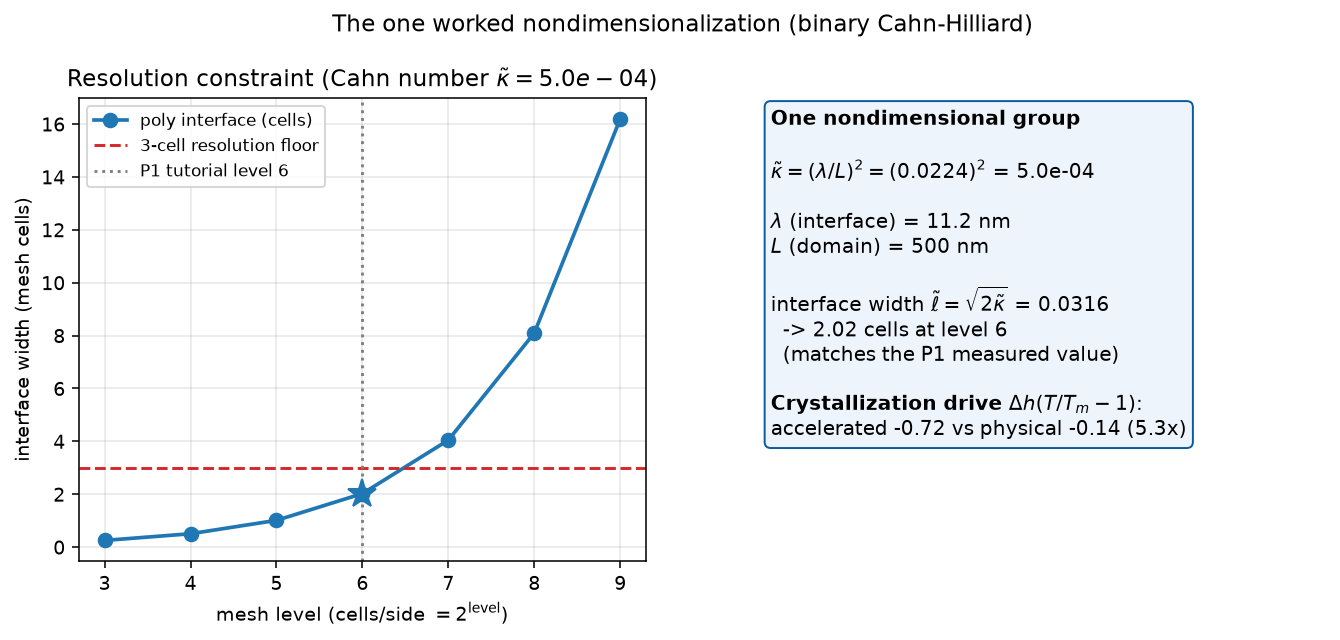
\includegraphics[width=\linewidth]{figures/p0_nondim.png}
  \caption{The one worked nondimensionalization. \emph{Left:} the interface
    width in mesh cells grows as $2^{\text{level}}$; the P1 tutorial level
    $\PzeroLevel$ (star) sits just below the $\PzeroTargetCells$-cell
    resolution floor, so the interface is marginally resolved --- a
    deliberate, documented tutorial trade-off. \emph{Right:} the single
    nondimensional group $\tilde\kappa=(\lambda/L)^2$ and the crystallization
    drive, computed by the harness and reproducing the P1 measured interface
    cells.}
  \label{fig:p0nondim}
\end{figure}

\section{Two crystallization conventions: p1 vs r14}

When crystallinity couples to composition (Chapter~\ref{ch:p7}), the Flory
interaction $\chi$ splits into \emph{four} matrices
$\chi_{aa},\chi_{ac},\chi_{ca},\chi_{cc}$ (amorphous/crystalline pairs), and
\textbf{the two bulk free energies in the code combine them differently} ---
a convention clash you must know before reading P6/P7. The \textbf{p1} bulk
uses a \emph{mutually-weighted} sum, so its four $\chi$ are \emph{absolute}
pair interactions; the \textbf{r14} bulk (the 2310.11844 form used by the
Allen--Cahn energetics) uses $\psi^2$-weighted \emph{increments} on top of
$\chi_{aa}$, so the same input means an \emph{increment} $\chi_{aa}+\chi_{ca}$
at the pure limit, not an absolute value. The two also use different
interpolation functions for the crystalline state. Chapter~\ref{ch:p7} gives
the exact formulas and \file{test\_chi\_limits.py} pins all four pure limits
for both conventions against the production evaluator (the P7 finding: quote
whether a crystalline $\chi$ is absolute or an increment, or the numbers are
meaningless).

\section{Three statements about ``the energy decreases''}

The gradient-flow guarantee ($\dd{F}{t}\le0$) is a statement about the
\emph{continuous} model. It does \emph{not} automatically survive
discretization, and the course is careful to keep three different claims
apart --- a distinction you will meet quantitatively in every energy plot:
\begin{enumerate}[nosep]
  \item \textbf{Thermodynamically motivated (continuous Lyapunov).} In the
        PDE, $\dd{F}{t}=-\intv M|\grad\mu|^2\dV\le0$ \emph{exactly}. A
        theorem about the model.
  \item \textbf{Discretely energy-stable.} Whether the \emph{time scheme}
        inherits $F^{n+1}\le F^{n}$ every step. A property of the
        discretization, not automatic --- it must be \emph{measured} (report
        the largest positive stepwise increment $\max_n(F^{n+1}-F^n)$).
  \item \textbf{One monotone run.} The particular trajectory you plotted
        went downhill. Necessary but not sufficient --- report the
        increment, do not just assert ``it looked monotone.''
\end{enumerate}
Chapter~\ref{ch:p1} makes all three concrete on a real run; the point of
naming them here is that ``the energy decreased'' is three different claims,
and only the first is free.

\section{Deliverable}

\begin{keybox}
\textbf{Your deliverable for this chapter} (template in
\file{physics/00\_model\_hierarchy/deliverable.md}):
\begin{enumerate}[nosep]
  \item A \textbf{one-page model map}: redraw Figure~\ref{fig:p0hierarchy}
        from memory, labelling for each concept (i) the order parameter(s)
        and whether each is conserved or non-conserved, (ii) the one
        ingredient it adds, and (iii) the free-energy term that ingredient
        introduces.
  \item A \textbf{completed parameter table}: take one real system from
        \file{materials/materials.yaml} and fill in all four columns ---
        dimensional value $+$ source, the nondimensional group it maps to,
        the numerical resolution it demands (minimum mesh level for
        $\ge\PzeroTargetCells$ interface cells), and any accelerated setting
        you would use for a quick run, \emph{labelled as accelerated}.
\end{enumerate}
Run \file{run.py} to reproduce the nondimensionalization numbers and check
your table against \file{outputs/p0/results.json}.
\end{keybox}

\section{Run it}

\begin{runbox}
\textbf{Run it.}
\begin{lstlisting}
cd physics/00_model_hierarchy
python run.py --config configs/p0.yaml --device cpu \
    --mode reference --output outputs/p0 --overwrite
python gen_figures.py --run-dir outputs/p0
\end{lstlisting}
The harness computes the worked nondimensionalization (the Cahn number, the
interface widths in cells, the minimum mesh level, and the accelerated-vs-
physical crystallization drive) from the dimensional inputs in
\file{configs/p0.yaml}, checks them against \file{baseline.yaml} (the
interface-cell counts must match the P1 tutorial), and records provenance in
\file{metadata.json}. \code{gen\_figures.py} renders the hierarchy map and
the nondimensionalization figure and writes \file{numbers/p0.tex}.
\end{runbox}

\section{Explore on your own}

\question{Take a second system from \file{materials.yaml} (say P3HT:PCBM at
$\chi=0.86$) and compute its FH curvature $f''(\bar\phi)$ at the symmetric
point. Is it spinodally unstable? What mesh level resolves its interface to
$\ge3$ cells?}

\question{Halve the domain $L$ at fixed interface $\lambda$. The Cahn number
$\tilde\kappa$ quadruples --- what happens to the interface-in-cells at fixed
mesh level, and to the minimum level you need? This is why a bigger physical
box is \emph{cheaper} to resolve, not more expensive.}

\question{For the crystallization drive $\Delta h(T/T_m-1)$, at what
temperature does the accelerated tutorial ($T=250$~K) overstate the physical
($T=500$~K) drive, and by how much? When is such an acceleration defensible,
and when does it change the physics rather than just the timing?}

\question{Classify each field in the moving-frame evaporation model
(\ref{ch:p5}) as conserved or non-conserved, and explain in which frame each
species' amount is actually conserved.}

\question{Write down which free-energy term is \emph{added} at each step of
Figure~\ref{fig:p0hierarchy}. Which additions change the dynamics type
(conserved $\leftrightarrow$ non-conserved), and which only add a term to
the same $F$?}

% ====================================================================
